\section*{13. Statistical Decision Theory}\label{statistical-decision-theory}

\subsection*{13.1 Preliminaries}\label{preliminaries}
\textbf{Decision theory} is a formal theory for comparing between
statistical procedures.
In the language of decision theory, a estimator is sometimes called a
\textbf{decision rule} and the possible values of the decision rule are
called \textbf{actions}.
We shall measure the discrepancy between \(\theta\) and \(\hat{\theta}\)
using a \textbf{loss function} \(L(\theta, \hat{\theta})\). Formally,
\(L\) maps \(\Theta \times \Theta\) into \(\R\).
The \textbf{risk} of an estimator \(\hat{\theta}\) is
\[
R(\theta, \hat{\theta}) = \EXP_{\theta} \left( L(\theta, \hat{\theta}) \right)
= \int L(\theta, \hat{\theta}(x)) f(x; \theta) dx
\]
When the loss function is squared error, then the risk is just the mean
squared error:
\[
R(\theta, \hat{\theta}) = \EXP_{\theta}(\hat{\theta} - \theta)^{2} = \MSE = \VAR_\theta(\hat{\theta}) + \text{bias}_\theta^{2}(\hat{\theta})
\]
In the rest of chapter, if the risk function is not specified, assume
the loss function is the squared error.

\subsection*{13.2 Comparing Risk
Functions}\label{comparing-risk-functions}
The \textbf{maximum risk} is
\[
\bar{R}(\hat{\theta}) = \sup_\theta R(\theta, \hat{\theta})
\]
and the \textbf{Bayes risk} is
\[
r(\pi, \hat{\theta}) = \int R(\theta, \hat{\theta}) \pi(\theta) d\theta
\]
where \(\pi(\theta)\) is a prior for \(\theta\).
An estimator that minimizes the maximum risk is called a \textbf{minimax
rule}. Formally, \(\hat{\theta}\) is minimax if
\[
R(\theta, \hat{\theta}) = \inf_{\bar{\theta}} \sup_\theta R(\theta, \hat{\theta})
\]
where the infimum is over all estimators \(\bar{\theta}\).
A decision rule that minimizes the Bayes risk is called a \textbf{Bayes
rule}. Formally, \(\hat{\theta}\) is a Bayes rule for prior \(\pi\) if
\[
R(\theta, \hat{\theta}) = \inf_{\bar{\theta}} r(\pi, \bar{\theta})
\]
where the infimum is over all estimators \(\bar{\theta}\).

\subsection*{13.3 Bayes Estimators}\label{bayes-estimators}
Let \(\pi\) be a prior. From Bayes' Theorem, the posterior density is
\[
f(\theta | x) = \frac{f(x | \theta) \pi(\theta)}{m(x)} = \frac{f(x | \theta) \pi(\theta)}{\int f(x | \theta) \pi(\theta) d\theta}
\]
where
\(m(x) = \int f(x, \theta) d\theta = \int f(x | \theta) \pi(\theta) d\theta\)
is the \textbf{marginal distribution} of \(X\). Define the
\textbf{posterior risk} of an estimator \(\hat{\theta}(x)\) by
\[
r(\hat{\theta} | x) = \int L(\theta, \hat{\theta}(x)) f(\theta | x) d\theta
\]

\textbf{Theorem 13.8}. The Bayes risk \(r(\pi, \hat{\theta})\) satisfies
\[
r(\pi, \hat{\theta}) = \int r(\hat{\theta} | x) m(x) dx
\]
Let \(\hat{\theta}(x)\) be the value of \(\theta\) that minimizes
\(r(\hat{\theta} | x)\). Then \(\hat{\theta}\) is the Bayes estimator.
\textbf{Proof}. We can rewrite the Bayes risk as:
\begin{align*}
r(\pi, \hat{\theta} &= \int R(\theta, \hat{\theta}) \pi(\theta) d\theta = \int \left( \int L(\theta, \hat{\theta}(x)) f(x | \theta) dx \right) \pi(\theta) d\theta \\
&= \int \int L(\theta, \hat{\theta}(x)) f(x, \theta) dx d\theta = \int \int L(\theta, \hat{\theta}(x)) f(\theta | x) m(x) dx d\theta \\
&= \int \left(\int L(\theta, \hat{\theta}(x) d\theta \right) m(x) dx = \int r(\hat{\theta} | x) m(x) dx
\end{align*}
If \(\hat{\theta} = \text{argmin}_\theta r(\hat{\theta} | x)\) then we
will minimize the integrand at every \(x\) and thus minimize the
integral \(\int r(\hat{\theta} | x)m(x) dx\).

\textbf{Theorem 13.9}. If
\(L(\theta, \hat{\theta}) = (\theta - \hat{\theta})^{2}\) then the Bayes
estimator is
\[
\hat{\theta}(x) = \int \theta f(\theta | x) d\theta = \EXP(\theta | X = x)
\]
If \(L(\theta, \hat{\theta}) = |\theta - \hat{\theta}|\) then the Bayes
estimator is the median of the posterior \(f(\theta | x)\). If
\(L(\theta, \hat{\theta})\) is zero-one loss, then the Bayes estimator
is the mode of the posterior \(f(\theta | x)\).
\textbf{Proof}. We will prove the Theorem for the squared error loss.
The Bayes rule \(\hat{\theta}\) minimizes
\(r(\theta | x) = \int (\theta - \hat{\theta}(x))^{2} f(\theta | x) d\theta\).
Taking the derivative of \(r(\hat{\theta} | x)\) with respect to
\(\hat{\theta}(x)\) and setting it to 0 yields the equation
\(2 \int (\theta - \hat{\theta}(x)) f(\theta | x) d\theta = 0\). Solving
for \(\hat{\theta}(x)\) we get the given estimator.

\subsection*{13.4 Minimax Rules}\label{minimax-rules}
The problem of Minimax Rules is complicated and a complete coverage of
that theory will not be attempted here, but a few key results will be
mentioned. Main takeaway message from this section: Bayes estimators
with a constant risk function are minimax.

\textbf{Theorem 13.11}. Let \(\hat{\theta}^\pi\) be the Bayes rule for
some prior \(\pi\):
\[
r(\pi, \hat{\theta}^\pi) = \inf_{\hat{\theta}} r(\pi, \hat{\theta})
\]
Suppose that
\[
R(\theta, \hat{\theta}^\pi) \leq r(\pi, \hat{\theta}^\pi) \;\text{for all } \theta
\]
Then \(\hat{\theta}^\pi\) is minimax and \(\pi\) is called a
\textbf{least favorable prior}.
\textbf{Proof}. Suppose that \(\hat{\theta}^\pi\) is not minimax. Then
there is another rule \(\hat{\theta}_{0}\) such that
\(\sup_\theta R(\theta, \hat{\theta}_{0}) \leq \sup_\theta R(\theta, \hat{\theta}^\pi)\).
Since the average of a function is always less than or equal to its
maximum, we have that
\(r(\theta, \hat{\theta}_{0}) \leq \sup_\theta R(\theta, \hat{\theta}_{0})\).
Hence,
\[
r(\theta, \hat{\theta}_{0}) \leq \sup_\theta R(\theta, \hat{\theta}_{0}) \leq \sup_\theta R(\theta, \hat{\theta}^\pi) \leq r(\pi, \hat{\theta}^\pi)
\]
which contradicts
\(r(\pi, \hat{\theta}^pi) = \inf_{\hat{\theta}} r(\pi, \hat{\theta})\).

\textbf{Theorem 13.12}. Suppose that \(\hat{\theta}\) is the Bayes rule
estimator with respect to some prior \(\pi\). Suppose further that
\(\hat{\theta}\) has constant risk: \(R(\theta, \hat{\theta}) = c\) for
some \(c\). Then \(\hat{\theta}\) is minimax.
\textbf{Proof}. The Bayes risk is
\(r(\pi, \hat{\theta}) = \int R(\theta, \hat{\theta}) \pi(\theta) d\theta = c\)
and hence \(R(\theta, \hat{\theta}) \leq r(\pi, \hat{\theta})\) for all
\(\theta\). Now apply Theorem 13.11.

\textbf{Theorem 13.15}. Let \(X_{1}, \dots, X_{n} \sim N(\theta, 1)\) and
let \(\hat{\theta} = \bar{X}\). Then \(\hat{\theta}\) is minimax
with respect to any well-behaved loss function. It is the only estimator
with this property.
\emph{Well-behaved means that the level sets must be convex and
symmetric about the origin. The result holds up to sets of measure 0.}

\subsection*{13.5 Maximum Likelihood, Minimax and
Bayes}\label{maximum-likelihood-minimax-and-bayes}
For parametric models that satisfy weak regularity conditions, the MLE
is approximately minimax. Consider squared error loss which is squared
bias plus variance. In parametric models with large samples, it can be
shown that the variance term dominates the bias so the risk of the MLE
\(\hat{\theta}\) roughly equals the variance:
\[
R(\theta, \hat{\theta}) = \VAR_\theta(\hat{\theta}) + \text{bias}^{2} \approx \VAR_\theta(\hat{\theta})
\]
\emph{Typically, the squared bias is of order \(O(n^{-2})\) while the
variance is of order \(O(n^{-1})\).}
As seen on the chapter on parametric models, the variance is
approximately:
\[
\VAR(\hat{\theta}) = \frac{1}{nI(\theta)}
\]
where \(I(\theta)\) is the Fisher information. Hence,
\[
n R(\theta, \hat{\theta}) \approx \frac{1}{I(\theta)}
\]
For any other estimator \(\theta'\), it can be shown that, for large
\(n\), \(R(\theta, \theta') \geq R(\theta, \hat{\theta})\). More
precisely,
\[
\lim_{\epsilon \rightarrow 0} \limsup_{n \rightarrow \infty} \sup_{|\theta - \theta'| < \epsilon} n R(\theta', \hat{\theta}) \geq \frac{1}{I(\theta)}
\]
This says that, in a local, large sample sense, the MLE is minimax. It
can also be shown that the MLE is approximately the Bayes rule.
In summary, in parametric models with large samples, the MLE is
approximately minimax and Bayes. There is a caveat: these results break
down when the number of parameters is large.

\subsection*{13.6 Admissibility}\label{admissibility}
An estimator \(\hat{\theta}\) is \textbf{inadmissible} if there exists
another rule \(\hat{\theta}'\) such that
\begin{align*}
R(\theta, \hat{\theta}') \leq R(\theta, \hat{\theta}) & \quad \text{for all } \theta \text{ and} \\
R(\theta, \hat{\theta}') < R(\theta, \hat{\theta}) & \quad \text{for at least one } \theta
\end{align*}
A prior has \textbf{full support} if for every \(\theta\) and every
\(\epsilon > 0\),
\(\int_{\theta - \epsilon}^{\theta + \epsilon} \pi(\theta) d\theta > 0\).

\textbf{Theorem 13.20 (Bayes' rules are admissible)}. Suppose that
\(\theta \subset \R\) and that \(R(\theta, \hat{\theta})\) is a
continuous function of \(\theta\) for every \(\hat{\theta}\). Let
\(\pi\) be a prior density with full support and let
\(\hat{\theta}^\pi\) be the Bayes' rule. If the Bayes risk is finite
then \(\hat{\theta}^\pi\) is admissible.
\textbf{Proof}. Suppose \(\hat{\theta}^\pi\) is inadmissible. Then there
exists a better rule \(\hat{\theta}\) such that
\(R(\theta, \hat{\theta}) \leq R(\theta, \hat{\theta}^\pi)\) for all
\(\theta\) and
\((\theta_{0}, \hat{\theta}) < R(\theta_{0}, \hat{\theta}^\pi)\) for some
\(\theta_{0}\). Let
\(v = R(\theta_{0}, \hat{\theta}^\pi) - R(\theta_{0}, \hat{\theta}) > 0\).
Since \(R\) is continuous, there is an \(\epsilon > 0\) such that
\(R(\theta, \hat{\theta}^\pi) - R(\theta_{0}, \hat{\theta}) > v/2\) for
all \(\theta \in (\theta_{0} - \epsilon, \theta_{0} + \epsilon)\). Now,
\begin{align*}
r(\pi, \hat{\theta}^pi) - r(\pi, \hat{\theta}) &= \int R(\theta, \hat{\theta}^\pi) \pi(\theta) d\theta - \int R(\theta, \hat{\theta}) \pi(\theta) d\theta \\
&= \int \left[ R(\theta, \hat{\theta}^\pi) - R(\theta, \hat{\theta})\right] \pi(\theta) d\theta \\
&\geq \int_{\theta_{0} - \epsilon}^{\theta_{0} + \epsilon} \left[ R(\theta, \hat{\theta}^\pi) - R(\theta, \hat{\theta})\right] \pi(\theta) d\theta \\
& \geq \frac{v}{2} \int_{\theta_{0} - \epsilon}^{\theta_{0} + \epsilon} \pi(\theta) d\theta \\
& > 0
\end{align*}
Hence \(r(\pi, \hat{\theta}^\pi) > r(\pi, \hat{\theta})\). This implies
that \(\hat{\theta}^\pi\) does not minimize \(r(\pi, \hat{\theta})\),
which contradicts the fact that \(\hat{\theta}^\pi\) is the Bayes rule.

\textbf{Theorem 13.21}. Let \(X_{1}, \dots, X_{n} \sim N(\mu, \sigma^{2})\).
Under squared error loss, \(\bar{X}\) is admissible.
The proof of this Theorem is very technical and ommitted. Outline: the
posterior mean is admissible for any strictly positive prior. Take the
prior to be \(N(a, b^{2})\). When \(b^{2}\) is very large, the posterior
mean is approximately equal to \(\bar{X}\).
In general, a rule may be minimax, admissible, both, or neither. Here
are some facts linking admissibility and minimaxity.

\textbf{Theorem 13.22}. Suppose that \(\hat{\theta}\) has constant risk
and is admissible. Then it is minimax.
\textbf{Proof}. The risk is \(R(\theta, \hat{\theta}) = c\) for some
constant \(c\). If \(\hat{\theta}\) were not minimax then there exists a
rule \(\hat{\theta}'\) that further reduces the risk,
\[
R(\theta, \hat{\theta}') \leq \sup_{\theta} R(\theta, \hat{\theta}') < \sup_{\theta} R(\theta, \hat{\theta}) = c
\]
But that would imply that \(\hat{\theta}\) is inadmissible.

\textbf{Theorem 13.23}. Let \(X_{1}, \dots, X_{n} \sim N(\theta, 1)\). Then,
under squared error loss, \(\hat{\theta} = \bar{X}\) is minimax.
\textbf{Proof}. According to Theorem 13.21, \(\hat{\theta}\) is
admissible. The risk of \(\hat{\theta}\) is \(1/n\) which is constant.
According to Theorem 13.22, it is also minimax.
Although miminax rules are not guaranteed to be admissible they are
``close to admissible''. Say \(\hat{\theta}\) is \textbf{strongly
inadmissible} if there is a rule \(\hat{\theta}'\) and an
\(\epsilon > 0\) such that
\(R(\theta, \hat{\theta}') < R(\theta, \hat{\theta}) - \epsilon\) for
all \(\theta\).

\textbf{Theorem 13.24}. If \(\hat{\theta}\) is minimax then it is not
strongly inadmissible.

\subsection*{13.7 Stein's Paradox}\label{steins-paradox}
Suppose that \(X \sim N(0, 1)\) and consider estimating \(\theta\) with
squared error loss. From the previous section we know that
\(\hat{\theta}(X) = X\) is admissible.
Now consider estimating two, unrelated quantities
\(\theta = (\theta_{1}, \theta_{2})\) and suppose that
\(X_{1} \sim N(\theta_{1}, 1)\) and \(X_{2} \sim N(\theta_{2}, 1)\)
independently, with loss
\(L(\theta, \hat{\theta}) = \sum_{j=1}^{2} (\theta_{j} - \hat{\theta}_{j})^{2}\).
Not surprisingly, \(\hat{\theta}(X) = X\) is again admissible, where
\(X = (X_{1}, X_{2})\).
Now consider the generalization to \(k\) normal means. Let
\(\theta = (\theta_{1}, \dots, \theta_{k})\), \(X = (X_{1}, \dots, X_{k})\) with
\(X_{i} \sim N(\theta_{i}, 1)\) (independently) and loss
\(L(\theta, \hat{\theta}) = \sum_{j=1}^{k} (\theta_{j} - \hat{\theta}_{j})^{2}\).
Stein astounded everyone when he proved that, if \(k \geq 3\), then
\(\hat{\theta}(X) = X\) is inadmissible. It can be shown that the
following estimator, known as the James-Stein estimator, has smaller
risk:
\[
\hat{\theta}_S(X) = \left(1 - \frac{k-2}{\sum_{i} X_{i}^{2}} \right)^+ X_{i}
\]
where \((z)^+ = \max \{z, 0\}\). This estimator shrinks the \(X_{i}\)s
towards 0. The message is that, when estimating many parameters, there
is great value in ``shrinking'' the estimates. This observation plays an
important role in modern nonparametric function estimation.

\subsection*{13.9 Exercises}
\textbf{13.9.1}. In each of the following models, find the Bayes risk
and the Bayes estimator, using squared error loss.
\textbf{(a)} \(X \sim \text{Binomial}(n, p)\),
\(p \sim \text{Beta}(\alpha, \beta)\).
\textbf{(b)} \(X \sim \text{Poisson}(\lambda)\),
\(\lambda \sim \text{Gamma}(\alpha, \beta)\).
\textbf{(c)} \(X \sim N(\theta, \sigma^{2})\) where \(\sigma^{2}\) is known
and \(\theta \sim N(a, b^{2})\).

\textbf{Solution}
We can determine the posterior distribution, since its proportional to
the likelihood times the prior,
\(f(\theta | X) \propto \mathcal{L}(\theta | X) f(\theta)\). But when
using the square loss, the Bayes estimator is the mean of the posterior
(from Theorem 13.9). So we can then get the Bayes estimator as
\(\hat{\theta} = \EXP[\theta | X]\).
\textbf{(a)}
\begin{align*}
f(\theta | X) &\propto \mathcal{L}(\theta | X) f(\theta) \\
&= \prod_{i = 1}^N \left( \binom{N}{X_{i}} p^{X_{i}}(1 - p)^{n - X_{i}} \right) \frac{p^{\alpha - 1}(1-p)^{\beta - 1}}{B(\alpha, \beta)} \\
& \propto p^{(\alpha - 1) + \sum_{i} X_{i}} (1 - p)^{(\beta - 1) + \sum_{i} (n - X_{i})} \\
&= p^{\left(\alpha + N \bar{X}_N \right) - 1} (1 - p)^{\left(\beta + N(n - \bar{X}_N) \right)- 1}
\end{align*}
So the posterior is proportional to, and drawn from, a Beta
distribution:
\[
\theta | X \sim \text{Beta}\left(\alpha + N \bar{X}, \beta + N(n - \bar{X}) \right)
\]
The mean of the Beta distribution with parameters \(\alpha_p, \beta_p\)
is \(\alpha_p / (\alpha_p + \beta_p)\), so the posterior mean (and the
Bayes estimator) is:
\[
\hat{\theta}(X) = \frac{\alpha + N \bar{X}}{\alpha + \beta + Nn}
\]
The Bayes risk for an arbitrary estimator \(\tilde{\theta}\), given a
prior \(\pi(\theta)\) that \(\theta \sim \text{Beta}(\alpha, \beta)\)
is:
\begin{align*}
r(\pi, \tilde{\theta}) 
&= \int R(\theta, \tilde{\theta}) \pi(\theta) d\theta 
\\
&= \int (\tilde{\theta} - \theta)^{2} \frac{\theta^{\alpha - 1}(1 - \theta)^{\beta - 1}}{B(\alpha, \beta)} d\theta 
\\
&= \tilde{\theta}^{2} \int \frac{\theta^{\alpha - 1}(1 - \theta)^{\beta - 1}}{B(\alpha, \beta)} d\theta
\\
&- 2 \tilde{\theta} \int \theta \frac{\theta^{\alpha - 1}(1 - \theta)^{\beta - 1}}{B(\alpha, \beta)} d\theta
\\
&+ \int \theta^{2} \frac{\theta^{\alpha - 1}(1 - \theta)^{\beta - 1}}{B(\alpha, \beta)} d\theta 
\\
&= \tilde{\theta}^{2} \EXP_\pi[1] - 2 \tilde{\theta} \EXP_\pi[\theta] + \EXP_\pi[\theta^{2}]
\\
&= \tilde{\theta}^{2} \cdot 1 - 2 \tilde{\theta} \EXP_\pi[\theta] + \VAR_\pi[\theta] + \EXP_\pi[\theta]^{2} 
\\ 
&= \tilde{\theta}^{2} - 2 \tilde{\theta} \frac{\alpha}{\alpha + \beta}
+ \frac{\alpha\beta + \alpha^{2}(\alpha + \beta + 1)}{(\alpha + \beta)^{2}(\alpha + \beta + 1)}
\end{align*}
Including the observations from \(X\), the prior is modified to a
different Beta distribution, replacing \(\alpha\) by
\(\alpha + N \bar{X}\) and \(\beta\) by
\(\beta + N(n - \bar{X})\).
\textbf{(b)}
\begin{align*}
f(\theta | X) &\propto \mathcal{L}(\theta | X) f(\theta) \\
&= \prod_{i = 1}^N \left( \frac{\lambda^X_{i} e^{-\lambda}}{X_{i}!} \right) \frac{\beta^\alpha}{\Gamma(\alpha)}\lambda^{\alpha - 1}e^{-\beta \lambda} \\
& \propto \lambda^{\sum_{i} X_{i}} e^{-N \lambda} \lambda^{\alpha - 1} e^{-\beta \lambda} \\
&= \lambda^{\left(\alpha + N \bar{X}\right) - 1} e^{-(\beta + N) \lambda}
\end{align*}
So the posterior is proportional to, and drawn from, a Gamma
distribution:
\[
\theta | X \sim \text{Gamma}\left(\alpha + N \bar{X}, \beta + N \right)
\]
The mean of the Gamma distribution with parameters \(\alpha_p, \beta_p\)
is \(\alpha_p / \beta_p\), so the posterior mean (and the Bayes
estimator) is:
\[
\hat{\theta}(X) = \frac{\alpha + N \bar{X}}{\beta + N}
\]
The Bayes risk for an arbitrary estimator \(\tilde{\theta}\), given a
prior \(\pi(\theta)\) that \(\theta \sim \text{Gamma}(\alpha, \beta)\)
is:
\begin{align*}
r(\pi, \tilde{\theta}) 
&= \int R(\theta, \tilde{\theta})\pi(\theta) d\theta 
\\
&= \int (\tilde{\theta} - \theta)^{2} \frac{\beta^\alpha}{\Gamma(\alpha)} \theta^{\alpha - 1}e^{-\beta \theta} d\theta 
\\
&= \tilde{\theta}^{2} \int \frac{\beta^\alpha}{\Gamma(\alpha)} \theta^{\alpha - 1}e^{-\beta \theta} d\theta
\\
& \quad
- 2 \tilde{\theta} \int \theta \frac{\beta^\alpha}{\Gamma(\alpha)} \theta^{\alpha - 1}e^{-\beta \theta} d\theta
\\
& \quad
+ \int \theta^{2}\frac{\beta^\alpha}{\Gamma(\alpha)} \theta^{\alpha - 1}e^{-\beta \theta} d\theta 
\\
&= \tilde{\theta}^{2} \EXP_\pi[1] - 2 \tilde{\theta} \EXP_\pi[\theta] + \EXP_\pi[\theta^{2}] 
\\
&= \tilde{\theta}^{2} \cdot 1 - 2 \tilde{\theta} \EXP_\pi[\theta] + \VAR_\pi[\theta] + \EXP_\pi[\theta]^{2} 
\\
&= \tilde{\theta}^{2} - 2 \tilde{\theta} \frac{\alpha}{\beta} + \frac{\alpha(\alpha + 1)}{\beta^{2}}
\end{align*}
Including the observations from \(X\), the prior is modified to a
different Gamma distribution, replacing \(\alpha\) by
\(\alpha + N \bar{X}\) and \(\beta\) by \(\beta + N\).
\textbf{(c)}
\begin{align*}
f(\theta | X) &\propto \mathcal{L}(\theta | X) f(\theta) 
\\
&= \prod_{i = 1}^N \left( \frac{1}{\sigma \sqrt{2 \pi}} e^{-\frac{1}{2} \left(\frac{X_{i} - \theta}{\sigma} \right)^{2}} \right) \frac{1}{a \sqrt{2 \pi}} e^{-\frac{1}{2} \left( \frac{\theta - a}{b}\right)^{2}} 
\\
& \propto \exp \left\{ -\frac{1}{2} \left( \sum_{i=1}^N \left( \frac{X_{i} - \theta}{\sigma}\right)^{2} + \left( \frac{\theta - a}{b}\right)^{2} \right) \right\} 
\\
& = \exp \left\{-\frac{1}{2} \left( \theta^{2} \left(\frac{N}{\sigma^{2}} + \frac{1}{b^{2}} \right) - 2 \theta \left( \frac{N \bar{X}}{\sigma^{2}} + \frac{a}{b^{2}} \right) + C\right) \right\} 
\\
& \propto \exp \left\{-\frac{1}{2} \left( \frac{Nb^{2} + \sigma^{2}}{\sigma^{2} b^{2}} \right)\left(\theta^{2} - 2\theta \left(\frac{N b^{2} \bar{X} + a \sigma^{2}}{N b^{2} + \sigma^{2}} \right) \right) \right\} 
\\
& \propto \exp \left\{-\frac{1}{2} \left( \frac{Nb^{2} + \sigma^{2}}{\sigma^{2} b^{2}} \right) \left(\theta - \left(\frac{N b^{2} \bar{X} + a \sigma^{2}}{N b^{2} + \sigma^{2}} \right) \right)^{2} \right\} 
\\
& = \exp \left\{-\frac{1}{2} \left(\frac{\theta - \left(\frac{N b^{2} \bar{X} + a \sigma^{2}}{N b^{2} + \sigma^{2}} \right)}{\sqrt{\frac{\sigma^{2} b^{2}}{Nb^{2} + \sigma^{2}}}} \right)^{2} \right\} 
\\
& = \exp \left\{-\frac{1}{2} \left(\frac{\theta - \bar{\theta}}{w} \right)^{2} \right\}
\end{align*}
where
\[
\bar{\theta} = \frac{\sigma^{2}}{\sigma^{2} + N b^{2}}a + \frac{Nb^{2}}{\sigma^{2} + Nb^{2}}\bar{X}
\quad \text{and} \quad
w^{2} = \frac{1}{N} \frac{1}{\frac{1}{\sigma^{2}} + \frac{1}{Nb^{2}}}
\]
So the posterior is proportional to, and drawn from, a Normal
distribution:
\[
\theta | X \sim N(\bar{\theta}, w^{2})
\]
The mean of the Normal distribution is \(\bar{\theta}\), so the
mean of the posterior (and the Bayes estimator) is:
\[
\hat{\theta}(X) = \frac{\sigma^{2}}{\sigma^{2} + N b^{2}}a + \frac{Nb^{2}}{\sigma^{2} + Nb^{2}}\bar{X}
\]
The Bayes risk for an arbitrary estimator \(\tilde{\theta}\), given a
prior \(\pi(\theta)\) that \(\theta \sim N(a, b^{2})\) is:
\begin{align*}
r(\pi, \tilde{\theta}) &= \int R(\theta, \tilde{\theta}) \pi(\theta) d\theta 
\\
&= \int (\tilde{\theta} - \theta)^{2} \frac{1}{b \sqrt{2 \pi}} \exp \left\{ -\frac{1}{2} \left(\frac{\theta - a}{b}\right)^{2} \right\} d\theta 
\\
&= \tilde{\theta}^{2} \int \frac{1}{b \sqrt{2 \pi}} \exp \left\{ -\frac{1}{2} \left(\frac{\theta - a}{b}\right)^{2} \right\} d\theta
\\
& \quad
- 2 \tilde{\theta} \int \theta \frac{1}{b \sqrt{2 \pi}} \exp \left\{ -\frac{1}{2} \left(\frac{\theta - a}{b}\right)^{2} \right\} d\theta
\\
& \quad
+ \int \theta^{2} \frac{1}{b \sqrt{2 \pi}} \exp \left\{ -\frac{1}{2} \left(\frac{\theta - a}{b}\right)^{2} \right\} d\theta 
\\
&= \tilde{\theta}^{2} \EXP_\pi[1] - 2 \tilde{\theta} \EXP_\pi[\theta] + \EXP_\pi[\theta^{2}] 
\\
&= \tilde{\theta}^{2} - 2 \tilde{\theta} \EXP_\pi[\theta] + \VAR_pi[\theta] + \EXP_\pi[\theta]^{2} 
\\
&= \tilde{\theta}^{2} - 2 \tilde{\theta} a + a^{2} + b^{2}
\end{align*}
Including the observations from \(X\), the prior is modified to a
different Normal distribution, replacing \(a\) with
\(\bar{\theta}\) and \(b^{2}\) with \(w^{2}\).

\textbf{Exercise 13.9.2}. Let
\(X_{1}, \dots, X_{n} \sim N(\theta, \sigma^{2})\) and suppose we estimate
\(\theta\) with loss function
\(L(\theta, \hat{\theta}) = (\theta - \hat{\theta})^{2} / \sigma^{2}\). Show
that \(\bar{X}\) is admissible and minimax.

\textbf{Solution}.
The risk for an estimator \(\hat{\theta}\) is the risk for the same
estimator using the mean squared error, but scaled by \(1 / \sigma^{2}\):
\[
R_L(\theta, \hat{\theta}) = \EXP_{\theta}[L(\theta, \hat{\theta})] 
= \EXP_{\theta}\left[\left( \frac{\theta - \hat{\theta}}{\sigma} \right)^{2} \right] 
= \frac{1}{\sigma^{2}} \EXP_{\theta}[ L_{\MSE}(\theta, \hat{\theta})]  
= \frac{1}{\sigma^{2}} R_{\MSE}(\theta, \hat{\theta})
\]
Since \(\bar{X}\) is admissible and minimax for the MSE loss
function, it follows it is also admissible and minimax for this rescaled
loss function.

\textbf{Exercise 13.9.3}. Let
\(\Theta = \{ \theta_{1}, \dots, \theta_{k} \}\) be a finite parameter
space. Prove that the posterior mode is the Bayes estimator under
zero-one loss.

\textbf{Solution}. The Bayes rule minimizes
\[
r(\hat{\theta} | x) = \int L(\theta, \hat{\theta}) f(\theta | x) d\theta = \sum_{i} I(\hat{\theta} \neq \theta_{i}) f(\theta_{i} | x) = 1 - \sum_{i} I(\hat{\theta} = \theta_{i}) f(\theta_{i} | x) = 1 - f(\hat{\theta} | X)
\]
The posterior probability \(f(\theta | X)\) is maximized on the
posterior mode, \(\hat{\theta} = \text{argmax}_\theta f(\theta | X)\),
so the posterior mode is also the Bayes estimator under zero-one loss.

\textbf{Exercise 13.9.4 (Casella and Berger)}. Let \(X_{1}, \dots, X_{n}\)
be a sample from a distribution with variance \(\sigma^{2}\). Consider
estimators of the form \(bS^{2}\) where \(S^{2}\) is the sample variance.
Let the loss function for estimating \(\sigma^{2}\) be
\[
L(\sigma^{2}, \hat{\sigma}^{2}) = \frac{\hat{\sigma}^{2}}{\sigma^{2}} - 1 - \log \frac{\hat{\sigma^{2}}}{\sigma^{2}}
\]
Find the optimal value of \(b\) that minimizes the risk for all
\(\sigma^{2}\).

\textbf{Solution}. For an estimator of the form
\(\hat{\sigma}^{2} = bS^{2}\), the risk is
\begin{align*}
R(\sigma^{2}, bS^{2}) &= \EXP_{\sigma^{2}}[ L(\sigma^{2}, bS^{2}) ]\\
&=\EXP_{\sigma^{2}}\left[\frac{bS^{2}}{\sigma^{2}} - 1 - \log b - \log S^{2} + \log \sigma^{2} \right] \\
&= \frac{b}{\sigma^{2}} \EXP_{\sigma^{2}}[S^{2}] - 1 -\log b - \EXP_{\sigma^{2}}[\log S^{2}] + \log \sigma^{2} \\
&= b - \log b + C
\end{align*}
where \(C\) does not depend on \(b\). The risk is minimized when the
derivative is zero, \(1 - 1/b = 0\), or \(b = 1\).

\textbf{Exercise 13.9.5 (Berliner, 1983)}. Let
\(X \sim \text{Binomial}(n, p)\) and suppose the loss function is
\[
L(p, \hat{p}) = \left(1 - \frac{\hat{p}}{p} \right)^{2}
\]
where \(0 < p < 1\). Consider the estimator \(\hat{p}(X) = 0\). This
estimator falls outside of the parameter space \((0, 1)\) but we will
allow this. Show that \(\hat{p}(X) = 0\) is the unique, minimax rule.

\textbf{Solution}.
For the estimator \(\hat{p}(X) = 0\), the loss function is always 1, and
so the risk is also always 1.
For any estimator \(\tilde{p}\) that falls within the parameter space
\((0, 1)\), we are interested in calculating its maximum risk,
\(\bar{R}(p, \tilde{p}) = \sup_p R(p, \tilde{p})\).
\begin{align*}
R(p, \tilde{p}) &= \EXP_p \left[\left(1 - \frac{\tilde{p}(X)}{p} \right)^{2}\right]\\
&=\EXP_p \left[1 + \frac{1}{p} (-2 \tilde{p}(X)) + \frac{1}{p^{2}} \tilde{p}(X)^{2} \right] \\
&= 1 + \frac{1}{p} (-2 \EXP_p[\tilde{p}(X)]) + \frac{1}{p^{2}} \EXP_p[\tilde{p}(X)^{2}]
\end{align*}
For a specific estimator, we have the expectations as constants,
\(a = \EXP_p[\tilde{p}(X)]\) and
\(b = \EXP_p[\tilde{p}(X)^{2}]\). We are interested in picking a
\(p \in (0, 1)\) such that this risk is greater than 1; we can always do
\(p = a / b < 2a / b\), since \(a > 0\) due to the open interval
constraint:
\begin{align*}
1 + \frac{1}{p} (-2a) + \frac{1}{p^{2}} b > 1 \\
\frac{1}{p} \left(-2a + \frac{1}{p} b \right) > 0 \\
p < \frac{2a}{b}
\end{align*}
Therefore, any estimator within the parameter space can produce a risk
greater than 1, and it is not minimax as the estimator \(\hat{p}(X)\)
produces a smaller maximum risk.

\textbf{Exercise 13.9.6 (Computer Experiment)}. Compare the risk of the
MLE and the James-Stein estimator by simulation. Try various values of
\(n\) and various vectors \(\theta\). Summarize your results.

\textbf{Solution}.
Plot the mean square error from running the simulation a large
number of times for \(k = 3, 10, 100, 1000\), assuming that \(\theta\)
is a vector of all ones.

\begin{python}
import numpy as np
from scipy.stats import norm
import matplotlib.pyplot as plt
from tqdm import tqdm_notebook
# MLE estimator: just return the original values
def mle(X):
    return X
# James-Stein estimator: shrink towards zero
def james_stein(X):
    assert len(X) > 2
    return np.maximum(1 - ((len(X) - 2) / sum(X**2)), 0) * X
# Calculates the mean square error between two sequences
def mse(X_pred, X):
    return ((X - X_pred)**2).mean()
\end{python}

\begin{python}
def plot_range(k, B=100000):
    error_mle = np.empty(B)
    error_js = np.empty(B)
    for i in tqdm_notebook(range(B)):
        theta = np.ones(k)
        X = norm.rvs(loc=1, scale=1, size=k)
        theta_hat_mle = mle(X)
        theta_hat_js = james_stein(X)
        error_mle[i] = mse(theta_hat_mle, theta)
        error_js[i] = mse(theta_hat_js, theta)
    plt.figure(figsize=(12, 8))
    plt.hist(error_mle, density=True, bins=100, histtype='step', 
             color='blue', label='MLE, k = ' + str(k))
    plt.hist(error_js, density=True, bins=100, histtype='step', 
             color='red', label='James-Stein, k = ' + str(k))
    plt.legend(loc='upper right')
    plt.show()
\end{python}

\begin{python}
plot_range(3)
plot_range(10)
plot_range(100)
plot_range(1000)
\end{python}

\begin{figure}[H]
\centering
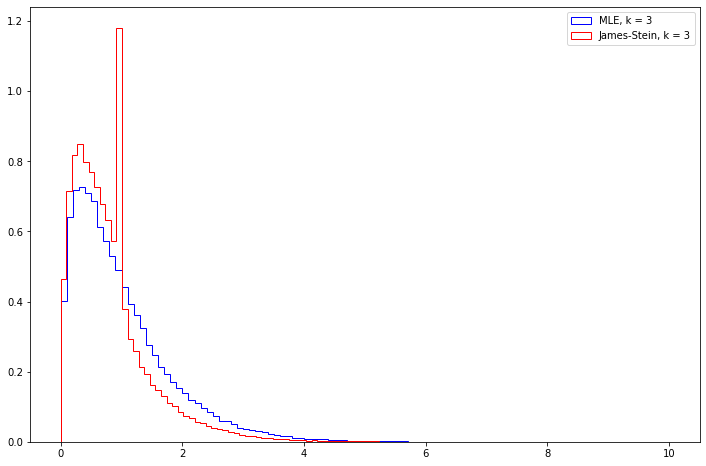
\includegraphics{Figure-13-01}
\end{figure}

\begin{figure}[H]
\centering
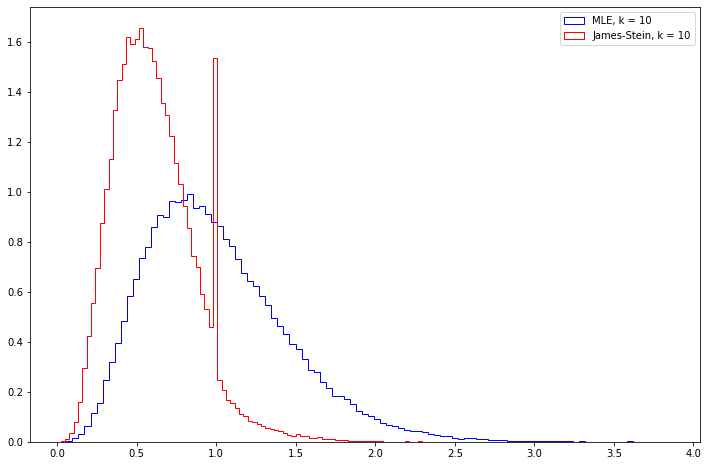
\includegraphics{Figure-13-02}
\end{figure}

\begin{figure}[H]
\centering
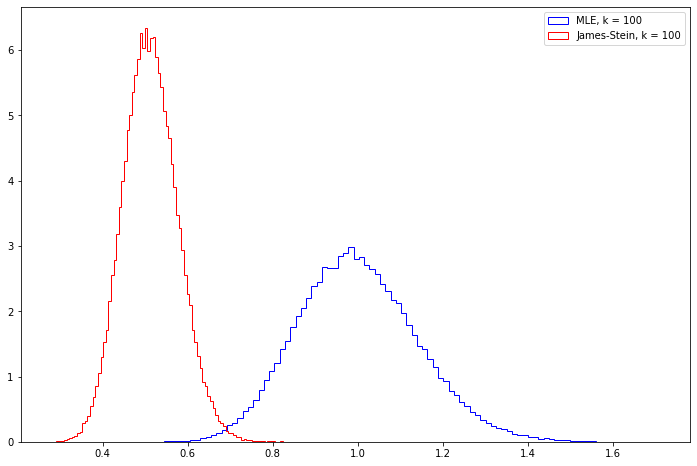
\includegraphics{Figure-13-03}
\end{figure}

\begin{figure}[H]
\centering
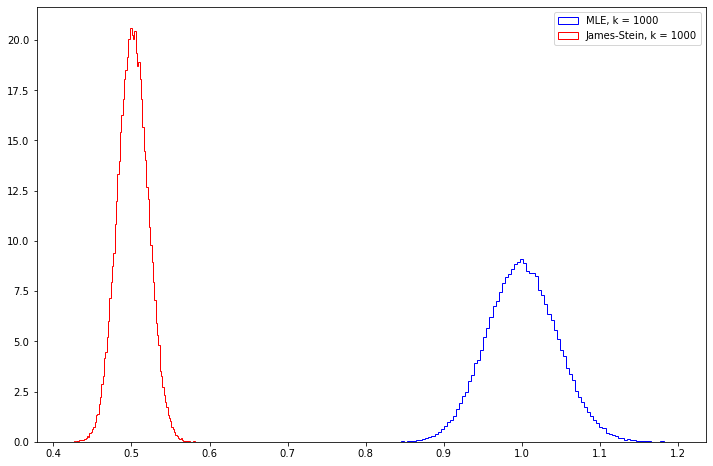
\includegraphics{Figure-13-04}
\end{figure}

Note that the James-Stein estimator seems to have its mean square error
go towards 0.5, while the MLE estimator has its error go towards 1.
